\chapter{Introduction}

\section{Background}
Looking at renting in the student accommodation industry, specifically on the ability to accurately forecast revenue using the data stored in the property management system (\cite{Jain2006IntellectualPerspective}). This will be done by using machine learning to predict under what circumstances a contract will not be fulfilled.

\vspace{5mm}

A contract made in advanced between the student (customer) and the company defines the services that will be sold (the room) as well as the start and end date of the tenancy and the fix price the service will be sold at. In the case of student accommodation this contract is usually made a few months in advanced, in some cases before the student has finalized there plan to attend a specific university. Because of this the student withholds the right to cancel the contract before it is paid. The inherit uncertainty of the contract means there is no way for the company to definitively measure what the occupancy and sales of a given property will be in advanced since they have to take on the risk. This problem is not specific to the student accommodation industry, this is a problem of revenue management first identified by the aviation industry in 1966  (\cite{Chiang2007AnResearch})

\vspace{5mm}


Having the ability to predict with some degree of certainty whether or not a booking is going to be cancelled would allow for more accurate decisions about revenue management to be made and overcome some of the risk created with contract based booking system. Doing this using machine learning means that overtime the accuracy of the predictions can increase with better understanding of the data, new iterations of modelling and evaluation of the actual outcome when compared with the predicted outcome. The ability for machine learning algorithm to make accurate predictions on a given outcome depends on the data available to it the amount of the data and the accuracy and usability of the data in, the case of booking management a lot of data is stored about each booking made. Meaning that it should be possible with the correct classification techniques to make accurate predictions on the outcome of the booking


\subsection{Problem Statement}

In total for the year 2020 to 2021, 25 percent of all 14363 bookings made where cancelled, this accounts for over 20 million pounds in revenue loss from customers who completed there booking then cancelled before the contract was payed. There are a number of different reasons that account for each booking being cancelled that range from impact caused due to COVID and students not receiving there target grades. In most of these cases the student will then chose to stay at different accommodation meaning the sale has been lost. Producing a model that is able to predict which of these bookings will be cancelled in real time would then allow the business to take actions to try and prevent the student from cancelling there booking. Being able to prevent just 10 percent of users from cancelling would therefore create a potential gain of 2 million in revenue per year.  

\vspace{5mm}

On a small scale it would be relatively easy for a human to identify the attributes common with bookings that would then be canceled, for example looking at the percentage of bookings canceled in the previous year. In this case however when the company operates over 70,000 beds across the world it is clear that no amount of human analysis would be able to take into account that many variables. 

\vspace{5mm}

\textbf{this paragraph is mostly a repeat of the 2nd paragraph}The fact that when a booking is made the student maintains the ability to cancel it up until a given time period for a given penalty means that it is the providers responsibility to account for the inherit uncertainty of the agreement. There's a number of different ways this problem can be solved that should take into account all of the possible variables, usually this is done by simply taking the number of bookings canceled in the previous year then using this number as an average to calculate the number of bookings likely to be canceled in the current year. The problem with this method is that it only takes into account one of the many variables (previous year figures) when in reality the business stores hundreds of data points on each of the bookings made.

It is for this reason I am attempting to solve this problem using machine learning

Since the dataset I am using is coming directly from the company in question and contains real data about students I have taken out all personal information I will be referring to students and properties only by there ID so that the company and students remain anonymous. 
    
\section{Aims and objectives}
The aim is to predict with some degree of certainty which of the bookings currently made and any new bookings will be cancelled by inputting all data points from the previous years bookings, I hope to produce a model that can classify a booking made into 2 distinct states, cancelled or not cancelled.

It is important to not just create a model that will predict which bookings will be cancelled but also to understand why bookings are cancelled by using the model to identify which features in the dataset have the most affect on weather or not the customer will cancel. Doing this is important in helping the company to make business decisions on the data to not only prevent the cancellation from occurring but to understand what actions can be taken that will reduce the number of cancellations made in the future.  

The first stage to any machine learning problem is obtaining accurate and clean data, in most cases (including this one), this is the hardest problem to solve as data is not usually stored in a way that makes it easy to read and analyse, most of the time data is stored  then never used. For this reason I am approaching the problem by building a data warehouse to properly store and analyse the data before building a classification model [\textbf{reference supporting why accurate data is important}]. This data warehouse will exist in the Azure cloud on top of Docker Containers with the code written in python, with the aim being to create a stream to import new booking data into the data warehouse hourly ensuring that it is stored in a way that makes it easy to use for model training

The aim is to integrate the classification model into the booking management system by creating a daily list of which customers are most likely to cancel there bookings to the managers of there respective properties along with the recommended actions to be taken to prevent the cancellation. Storing the data of the actions taken and weather or not it was successful can then be used to improve future iterations of the model




\section{Solution approach}

\begin{itemize}
\item talk about the split of data in the training set, 75 percent of the training data contains bookings that are not cancelled and 25 percent cancelled 
\end{itemize}


To understand what the best way to approach the solution to the problem would be I started by working with employees in the company to gain a better understanding of what kind of results would be most effective and what are the actions that can be take to have the best chance of preventing a cancellation from being made at the level of an individual booking. It is important the results can be displayed in a way that is easy for employees to understand so that actions can be taken. I found that the best way to display the results of the model would be to create a table that ranked bookings by highest probability of cancellation. Another feature I found to be important is the ability to retrain the model on new data and adjust the hyper tuning parameters.

To account for the multiple different stages involved in the Data Mining process I am going to be using the CRISP-DM model (\cite{WirthCRISP-DM:Mining}) to break down the problem into 6 specific stages \textbf{reference the figure}, these stages are business understanding, data understanding, data preparation, modeling, evaluation and deployment.

According to current research, CRISP-DM is the most commonly used data-mining model due to its numerous advantages, which solved existing data-mining problems. 


\vspace{5mm}


 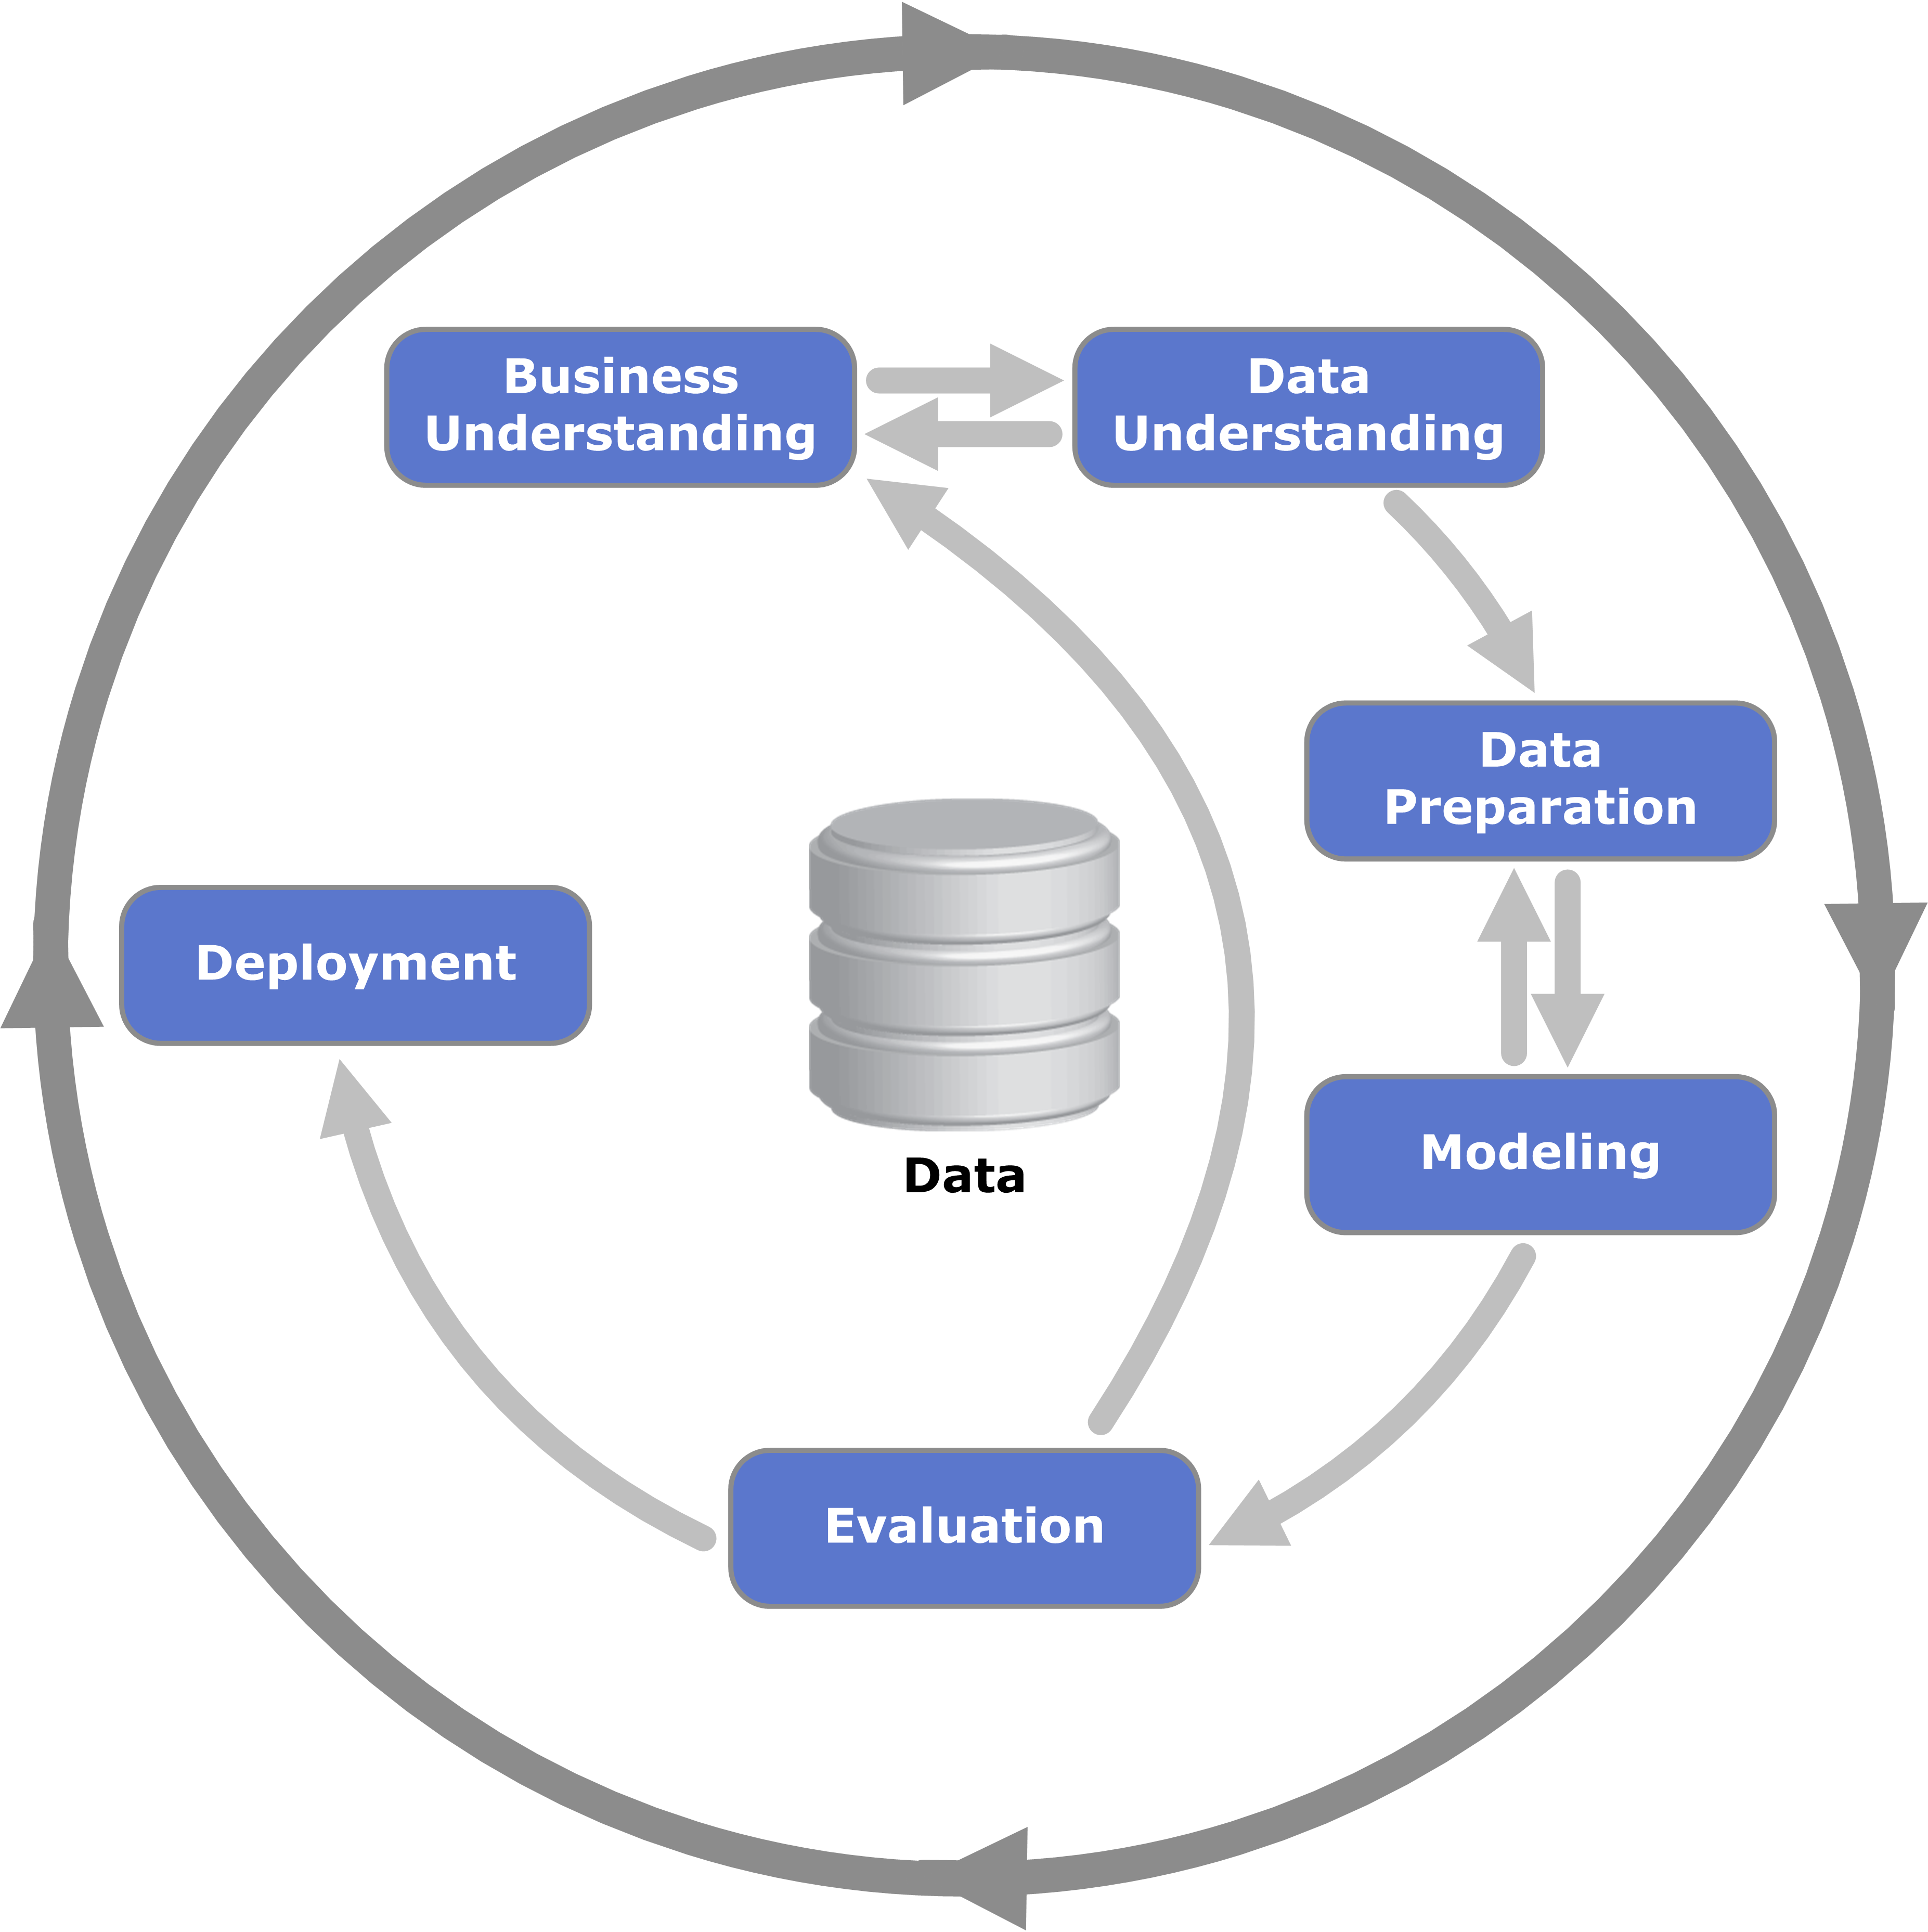
\includegraphics[width=10cm]{figures/CRISPDM_Process_Diagram.png}
 



I will be creating a model using the Azure ML studio to find if it is able to make accurate predictions on the data. I am using Azure ML because it provides the functionality to deploy models onto a cloud environment and significantly speeds up the process of model development . It also allows for easier retraining on the model after the evaluation stage while testing a number of different regression models each time and selecting the one with the highest accuracy.

The intended outcome of this research is to have the ability to rank bookings by the probability of them being cancelled, providing a platform to integrate the model results into the companies booking system. Doing this would allow the company to have the ability to input whether or not the prediction was correct. The model would then be able to be retrained based off the outcomes of the predictions, over time allowing for the models accuracy to be increased. 

In order for the solution of this problem to be useful, the solution method has to be fast and dynamic. Cancellation prediction needs to be in a time-frame that allows for actions to be taken to prevent the cancellation. Predicting the cancellation too late would not produce as useful information. Using azure ml can allow for a fast and dynamic method of predicting cancellations. 

One of the problems that needed to be solve was how to get access to data that is suitable for machine learning. This aspect consistently requires more time as seen in previous literature (\textbf{reference).} To perform machine learning, data needs to be accessible in a suitable format and stored appropriately. The current booking system behind the dataset in this research does not store the data in a way that is suitable for use in machine learning. Building a data warehouse allows for the data to be converted into an appropriate format for machine learning problems. An important aspect involves the ability of the data warehouse to update upon new bookings and allow instant access to the data, a feature of the data warehouse using azure cloud which was used in this project. 

The main technology used throughout the process will be Azure ML studio as a framework to encapsulate all of the tools needed to complete a machine learning project, it allows for direct connection to the database for accessing the data through integrated Jupiter Notebooks. Use of Jupiter Notebooks in Python provides an environment for all of the data cleaning and preparation stages that need to be performed entirely within the azure cloud. The modeling stages are done in the same way by importing the AzureML Python SDK into the Jupiter Notebook. The Experiment class (azureml.core.experiment.Experiment) in the SDK is used to store and run the models within a logical resource group with the ability to add and remove different modeling iterations form the experiment as well as viewing the results, when a model is configured through AutoMLConfig (azureml.train.automl.automlconfig.AutoMLConfig) it is then added to the experiment and the run is executed in the cloud. 

\begin{itemize}
\item Doing this process in the cloud helps to solve the the GDPR related problem of data access as the data is never stored on the local computer 
\end{itemize}
